\documentclass[a4paper,oneside,11pt]{report}
\usepackage[cm]{fullpage}
\usepackage{lmodern,amsmath,amssymb}
\usepackage{a4wide}
\setlength{\marginparwidth}{3cm}
\setlength{\topmargin}{0cm}
\setlength{\voffset}{0cm}
\setlength{\headsep}{0cm}
\title{ME 603 (FE for Biosmechanics) - Lab MSK}
\author{Debabrata Auddya}
%\usepackage{etoolbox}
%\preto\equation{\setcounter{equation}{0}}
%\makeatletter
%\pretocmd\start@gather{\setcounter{equation}{0}}{}{}
%\pretocmd\start@align{\setcounter{equation}{0}}{}{}
%\pretocmd\start@multline{\setcounter{equation}{0}}{}{}
%\makeatother
\usepackage{listings}
\usepackage{color}
\usepackage{dsfont}
\usepackage{footmisc}
\usepackage{verbatim}
\usepackage{smartdiagram}
\setlength{\marginparwidth}{0cm}
\setlength{\topmargin}{0cm}
\setlength{\voffset}{0cm}
\setlength{\headsep}{0cm}
\definecolor{dkgreen}{rgb}{0,0.6,0}
\definecolor{gray}{rgb}{0.5,0.5,0.5}
\definecolor{mauve}{rgb}{0.58,0,0.82}
\lstset{frame=tb,
	language=Java,
	aboveskip=3mm,
	belowskip=3mm,
	showstringspaces=false,
	columns=flexible,
	basicstyle={\small\ttfamily},
	numbers=none,
	numberstyle=\tiny\color{gray},
	keywordstyle=\color{blue},
	commentstyle=\color{dkgreen},
	stringstyle=\color{mauve},
	breaklines=true,
	breakatwhitespace=true,
	tabsize=3
}
\begin{document}
\maketitle
\section*{Part I}
\subsection*{1. Which degrees of freedom enable ankle
inversion/eversion?}
subtalar\_angle\_r
\subsection*{2. To tilt the platform in the sagittal plane
would you change platform\_ry
or platform\_rz?}
platform\_rz
\subsection*{3. Why do you think the mtp\_angle\_r
coordinate in the model is locked?}	
This is because the joint is under-actuated.
\section*{Part II}
\subsection*{1. What is the maximum subtalar angle during the drop landing?}
0.407 radians (23.319$^\circ$)
\subsection*{2. Would an ankle inversion injury have occurred during this landing? According to previous research (Siegler et al., 1990; Lapointe et al., 1997), angles larger than 25 degrees may cause injury.}
It is unlikely that an injury would have occurred during this landing as the maximum subtalar angle during the drop landing is lesser than 25$^\circ$ (0.436 radians)
\section*{Part III}
\subsection*{1. You have now simulated three different drop-landing conditions: without an AFO, with a soft AFO, and with a stiffer AFO. What differences in peak ankle inversion do you observe between the simulations?}
0.407 radians (23.319$^\circ$- Without AFO)
\\
0.688 radians (39.419$^\circ$ - SoftAFO)
\\
0.326 radians (18.678$^\circ$ - StiffAFO) \\
So we see that the peak angle for stiff AFO is the least and maximum for soft AFO. 
\subsection*{2. Could this AFO mitigate ankle inversion injuries?}
The StiffAFO could indeed prevent ankle injuries having ankle inversion angle much lesser than the permissible limit for injury. 
\section*{Appendix}
\subsection*{Angle Inversion Diagrams}
\begin{figure}[htb]
	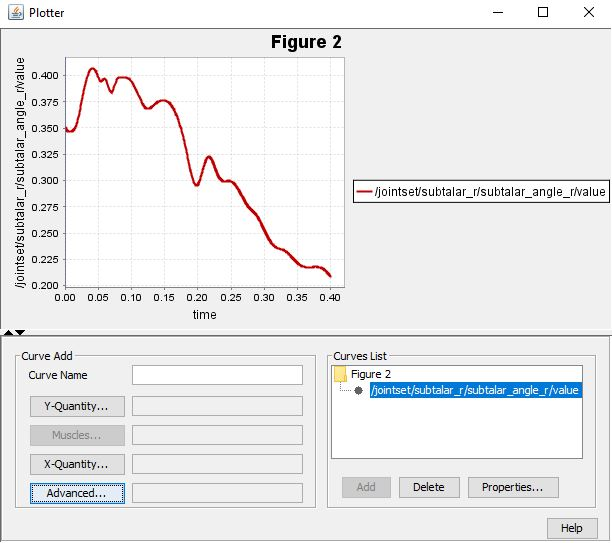
\includegraphics[width=0.4\textwidth]{ME603-MSK-PartOne.JPG}
	\caption{Without AFO}
	\label{fig:WithoutAFO}
\end{figure}
\begin{figure}[htb]
	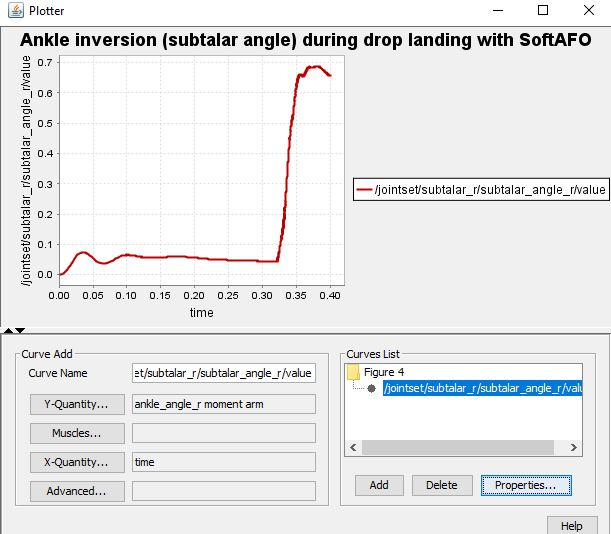
\includegraphics[width=0.4\textwidth]{ME603-MSK-SoftAFO.JPG}
	\caption{SoftAFO}
	\label{fig:SoftAFO}
\end{figure}
\begin{figure}[htb]
	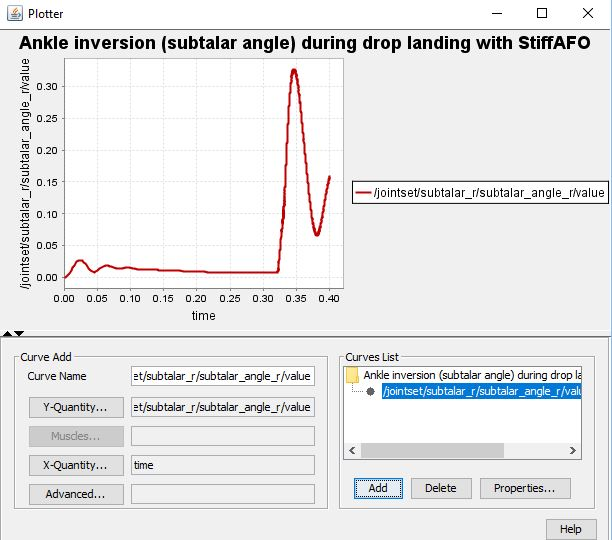
\includegraphics[width=0.4\textwidth]{ME603-MSK-StiffAFO.JPG}
	\caption{StiffAFO}
	\label{fig:StiffAFO}
\end{figure}
\end{document}
